%% Elsevier elsarticle template for NIM-A submission
%% Numeric-reference version

\documentclass[preprint,12pt]{elsarticle}
% If the editor requests a double-spaced review version, switch to:
% \documentclass[preprint,review,12pt]{elsarticle}

%% Other optional journal layouts:
%% \documentclass[final,1p,times]{elsarticle}
%% \documentclass[final,1p,times,twocolumn]{elsarticle}
%% \documentclass[final,3p,times]{elsarticle}
%% \documentclass[final,3p,times,twocolumn]{elsarticle}
%% \documentclass[final,5p,times]{elsarticle}
%% \documentclass[final,5p,times,twocolumn]{elsarticle}

\usepackage{graphicx}
\usepackage{multirow}
\usepackage{amsmath,amssymb,amsfonts}
\usepackage{amsthm}
\usepackage{booktabs}
\usepackage{array}
\usepackage{textcomp}
\usepackage{xcolor}
\usepackage{float}
\usepackage[section]{placeins}
\usepackage[hidelinks]{hyperref} % keep this near the end for clickable refs
\usepackage{microtype}
\usepackage{svg}
% Optional: line numbers for review
% \usepackage{lineno}
% \linenumbers

% ---------------- Figure / float tuning ----------------
\setcounter{topnumber}{3}
\setcounter{bottomnumber}{2}
\setcounter{totalnumber}{5}
\renewcommand{\topfraction}{0.9}
\renewcommand{\bottomfraction}{0.75}
\renewcommand{\textfraction}{0.08}
\renewcommand{\floatpagefraction}{0.8}

\setlength{\textfloatsep}{12pt plus 2pt minus 4pt}
\setlength{\floatsep}{10pt plus 2pt minus 2pt}
\setlength{\intextsep}{10pt plus 2pt minus 2pt}

\raggedbottom

\biboptions{numbers,sort&compress}

\journal{Nuclear Instruments and Methods in Physics Research Section A: Accelerators, Spectrometers, Detectors and Associated Equipment}

\begin{document}

\begin{frontmatter}

\title{Design and prototyping of the shim coil system for the TUCAN EDM experiment}

\author[uwinnipeg,umanitoba]{Amala Jaison\corref{cor1}}
\ead{amalajaison@gmail.com}

\author[uwinnipeg,carleton]{Shomi Ahmed\corref{cor1}}
\ead{ShomiAhmed@cunet.carleton.ca}

\author[triumf]{Derek Fujimoto\corref{cor1}}
\ead{dfujimoto@triumf.ca}

\author[uwinnipeg]{Modeste Katotoka\corref{cor1}}
\ead{modeste2016@outlook.com}

\author[uwinnipeg]{Jeffery W. Martin\corref{cor1}}
\ead{j.martin@uwinnipeg.ca}

\author[uwinnipeg]{Mark McCrea\corref{cor1}}
\ead{mark.mccrea@gmail.com}

\author[umanitoba]{Tahereh Mohammadi\corref{cor1}}
\ead{tmohammadi@triumf.ca}

\cortext[cor1]{Corresponding authors.}

\affiliation[uwinnipeg]{
  organization={Department of Physics, The University of Winnipeg},
  addressline={515 Portage Avenue},
  city={Winnipeg},
  state={MB},
  postcode={R3B 2E9},
  country={Canada}
}

\affiliation[umanitoba]{
  organization={Department of Physics and Astronomy, University of Manitoba},
  addressline={30A Sifton Road},
  city={Winnipeg},
  state={MB},
  postcode={R3T 2N2},
  country={Canada}
}

\affiliation[carleton]{
  organization={Carleton University},
  city={Ottawa},
  state={ON},
  country={Canada}
}

\affiliation[triumf]{
  organization={TRIUMF},
  addressline={4004 Wesbrook Mall},
  city={Vancouver},
  state={BC},
  postcode={V6T 2A3},
  country={Canada}
}

\begin{abstract}
Neutron electric dipole moment (nEDM) experiments require highly
uniform magnetic fields to preserve spin coherence during long storage
and precession times. The design and characterization of a prototype
square shim coil design developed for the TUCAN EDM experiment are
presented. The shim system consists of a 54-coil cubic array
(3$\times$3 coils per cube face) driven by a modular 64-channel
bipolar current supply.  The system is characterized inside the
magnetically shielded room using three-axis fluxgate scans along a
central axis.  The system qualitatively reproduces expected field
profiles for each coil, and for combinations of coils use to generate
harmonics of the magnetic field.  The coil currents for the harmonics
are calculated from a COMSOL simulation, and fluxgate scans compare
well with the expectations of the same simulation.  The results are a
step toward shimming the magnetic field and imply that the system
should be able provide the required field homogeneity.  ***NEED
NUMERICAL RESULTS***
\end{abstract}

\begin{keyword}
neutron electric dipole moment \sep magnetic shimming \sep shim coils
\sep magnetic field gradients \sep fluxgate magnetometer \sep
magnetically shielded room
\end{keyword}

\end{frontmatter}

\section{Introduction}\label{sec1}

The TUCAN EDM experiment aims to measure the neutron electric dipole
moment (nEDM) with a statistical uncertainty
$\sigma=10^{-27}~e\,\mathrm{cm}$ \cite{bib:npn}. In order to measure
the electric dipole moment (EDM) of the neutron $d$, ultracold
neutrons (UCNs) are stored in a bottle, and their spin precession
frequencies
\begin{equation}
\nu_\pm=\frac{2}{\hbar}(\mu B\pm dE)
\end{equation}
are measured in parallel ($+$) and antiparallel ($-$) configurations
of applied DC electric $E$ and magnetic $B$ fields.  Here, $\mu$ is
the magnetic dipole moment of the neutron.

Magnetic-field nonuniformities in nEDM experiments can lead to UCN
depolarization, and systematic frequency shifts in both the $^{199}$Hg
comagnetometer used in nEDM experiments, and the neutron frequency
itself~\cite{pendlebury2015,bib:Abel2019,bib:Abel2020CsMag,bib:Abel2022Mapping}.
Both effects are ultimately related to spin
relaxation\cite{bib:PignolRoccia2012,bib:Pignol2015SpinRelaxation,pendlebury2015}
The neutron depolarization caused by magnetic inhomogeneity results
from dephasing of the neutron spins.  As will be discussed, it results
mostly a gravitational effect.  Because the UCN kinetic energies are
so small ($\lesssim 300$~neV), neutrons of a lower kinetic energy will
preferentially sample the bottom of the precession chamber.  As a
result, neutrons of different energies will have spins that precess at
different average rates, due to imperfect motional averaging.  This
places a requirement on magnetic homogeneity which was the principal
requirement for the shim coils to address.

The dephasing results in a reduction in the visibility $\alpha$ of the
nuclear magnetic resonance signal, which normally has a
free-precession period of about $T=180$~s.  The visibility is the
degree of polarization of the neutrons after the NMR sequence has been
completed.  The visibility enters directly into the statistical
uncertainty $\sigma(d_n)$ of the nEDM experiment
\begin{equation}
\sigma(d_n)=\frac{\hbar}{2\alpha TE\sqrt{N}},
\end{equation}
where $N$ is the total number of neutrons counted at the end of the
NMR sequence.  Since the uncertainty is proportional to $T$ and
$\alpha$, it is crucially important that spin-coherence be maintained
over long periods of time.

A large magnetically shielded room (MSR) has been developed for the
TUCAN experiment to reduce external magnetic-field fluctuations and
provide a magnetically quiet environment for the
measurement~\cite{bib:msr_rsi}.  Within the shielded environment, the
expected dominant inhomogeneity is expected to arise from the remanent
magnetic fields after degaussing of the MSR.  In the previous best
nEDM experiment, this gave rise to a 3~nT inhomogeneity inside the
magnetic shield~\cite{bib:find-it}.  We used this level of
inhomogeneity as a guideline to design our shim coils, in advance of
having constructed the MSR.

Other uses of the shim coils are to provide various harmonic
components of the magnetic field $G_{\ell m}$, which play a role in
systematic frequency shifts, mostly of the $^{199}$Hg comagnetometer,
which lead to a false EDM signal~\cite{bib:Abel2019-I-think}.  The
coils can be used provide specific harmonics, and the resultant effect
on the false EDM measured.  The PSI nEDM experiment used this
technique up to order $\ell=3$.  Careful mapping of the magnetic field
to order $\ell=7$ was crucial to understand and correct
gradients~\cite{bib:Abel2022Mapping}.

In dual-cell nEDM experiments, the shim coils can be also used to
match the average magnetic field in the upper and lower measurement
cells.  This is needed so that the same $B_1$ coil can be used for the
NMR techniques needed for the two cells, and have the central
frequency be more-or-less the same.  This is particularly challenging
for the Ramsey-resonance technique used in these experiments.
Typically, the experiments are operated at a $B_0$ field of 1~$\mu$T,
corresponding to a neutron spin precession (Larmor) frequency of about
30~Hz.  The free-precession time of the neutrons approaches 180~s,
corresponding to a resonance width of 6 mHz, and the control of the
upper/lower cell matching condition must be significantly better than
the width ($\lesssim 100~\mu$Hz).

In our studies, matrix methods are used to determine current setpoints
for a desired magnetic field distribution.  Previous similar
techniques have focused on controlling the magnetic field external to
MSRs in active feedback systems, to improve the magnetic shielding
factor and overall stability of the shielded field
\cite{bib:franke-thesis,bib:rawlik-thesis,bib:shomi-thesis,bib:rawlik-amjphys,bib:abel-epjc-2023,bib:arxiv2601.22960}.
The techniques were adapted to the problem of internal magnetic field
shimming.  This is not a new usage of matrix techniques, but the
application to internal shimming is not often discussed in detail in
the literature.

This paper outlines the design considerations for the TUCAN EDM shim
coil system, design process, prototype design, and initial results
from the prototype using a primitive mapper using a fluxgate
magnetometer.  While the design originally used free-space calculation
techniques, the final results use COMSOL simulations to decide the
currents to produce the desired fields, and the fields are compared
with the same simulations.


\section{Design requirements}\label{sec2}

A primary purpose of the shim coils is to preserve the visibility
$\alpha$ of the neutron spin over long free-precession times.  The two
principal limitations on the neutron spin-relaxation are
gravitationally enhanced depolarization and intrinsic
depolarization~\cite{bib:Abel2019}. Gravitationally enhanced
depolarization arises because neutrons with different kinetic energies
sample different heights in the axially symmetric measurement cell.
In the presence of a vertical magnetic gradient, different mean
heights precess at different rates. The process is reversible, in the
sense that a spin-echo sequence can restore the visibility.  Intrinsic
depolarization is an irreversible dephasing within an energy group;
neutrons of the same energy, moving within an inhomogeneous magnetic
field, precess at different rates because they follow different
trajectories within the cell.

In a first-order gradient model~\cite{bib:Abel2019}, gravitationally
enhanced depolarization results in the following dependence of
visibility with free-precession time $T$
\begin{equation}
  \alpha_{\rm grav}=\alpha_0-\frac{1}{2}\gamma_n^2 G_{1,0}^2 {\rm Var}[\bar{z}] T^2,
  \label{eq:alphagrav}
\end{equation}
where $\gamma_n$ is the neutron gyromagnetic ratio, $G_{1,0}$ is the
first-order vertical gradient of $B_z$ in the harmonic-gradient
description used for nEDM magnetic-field analyses
\cite{bib:Abel2019,bib:Abel2022Mapping}, and ${\rm Var}[\bar{z}]$ is
the variance of the average $z$ positions for each neutron
energy. Intrinsic depolarization within an energy group can be
described using the ``intuitive model'' of
Ref.~\cite{bib:Harris2014GravitationalDepolarization,bib:Abel2019}
\begin{equation}
  \frac{1}{T_{2,\rm mag}}=
  \frac{8R^3\gamma_n^2}{9\pi v}\left(G_{1,-1}^2+G_{1,1}^2\right)
  +\frac{\mathcal{H}^3\gamma_n^2}{16v}G_{1,0}^2,
  \label{eq:intrinsic}
\end{equation}
with the corresponding visibility
\begin{equation}
  \alpha_{\rm mag}=\alpha_0\exp\left(-\frac{T}{T_{2,\rm mag}}\right).
  \label{eq:alphamag}
\end{equation}
In Eq.~(\ref{eq:intrinsic}), $T_{2,\rm mag}$ is the magnetic
contribution to the transverse spin-relaxation time, $v$ is the
neutron speed, $R$ is the cell radius, and $G_{1,1}$ and $G_{1,-1}$
are the first-order transverse gradients.  The quantity $\mathcal{H}$
is the effective height, defined as the maximum height attained by
neutrons of a given energy \cite{bib:afach-prd-92-052008-2015}.  If
the neutron kinetic energy is $E$, its maximum height in free space is
$\epsilon=\frac{E}{mg}$.  For neutrons trapped within the measurement
cell of height $H$, the effective height $\mathcal{H}$ is the lesser
of $H$ and $\epsilon$.

Both Eqs. (\ref{eq:alphagrav}) and (\ref{eq:alphamag}) were compared
with data on neutron visibility from PSI in Ref.~\cite{bib:Abel2019}
and found to agree well with data.  Eq.~(\ref{eq:alphagrav}) was found
to be valid in a more limited range of $G_{1,0}\lesssim 30$~pT/cm.

In Fig.~\ref{fig:g10_visibility}, we graph both
Eqs.~(\ref{eq:alphagrav}) and (\ref{eq:alphamag}) using parameters
relevant to the TUCAN EDM experiment.  This shows that gravitationally
enhanced depolarization (via $G_{1,0}$) tends to limit the visibility
$\alpha$ more stringently, for vertical gradients.  The parameters
used in making the graph are...???
\begin{figure}[tbp]
  \centering
  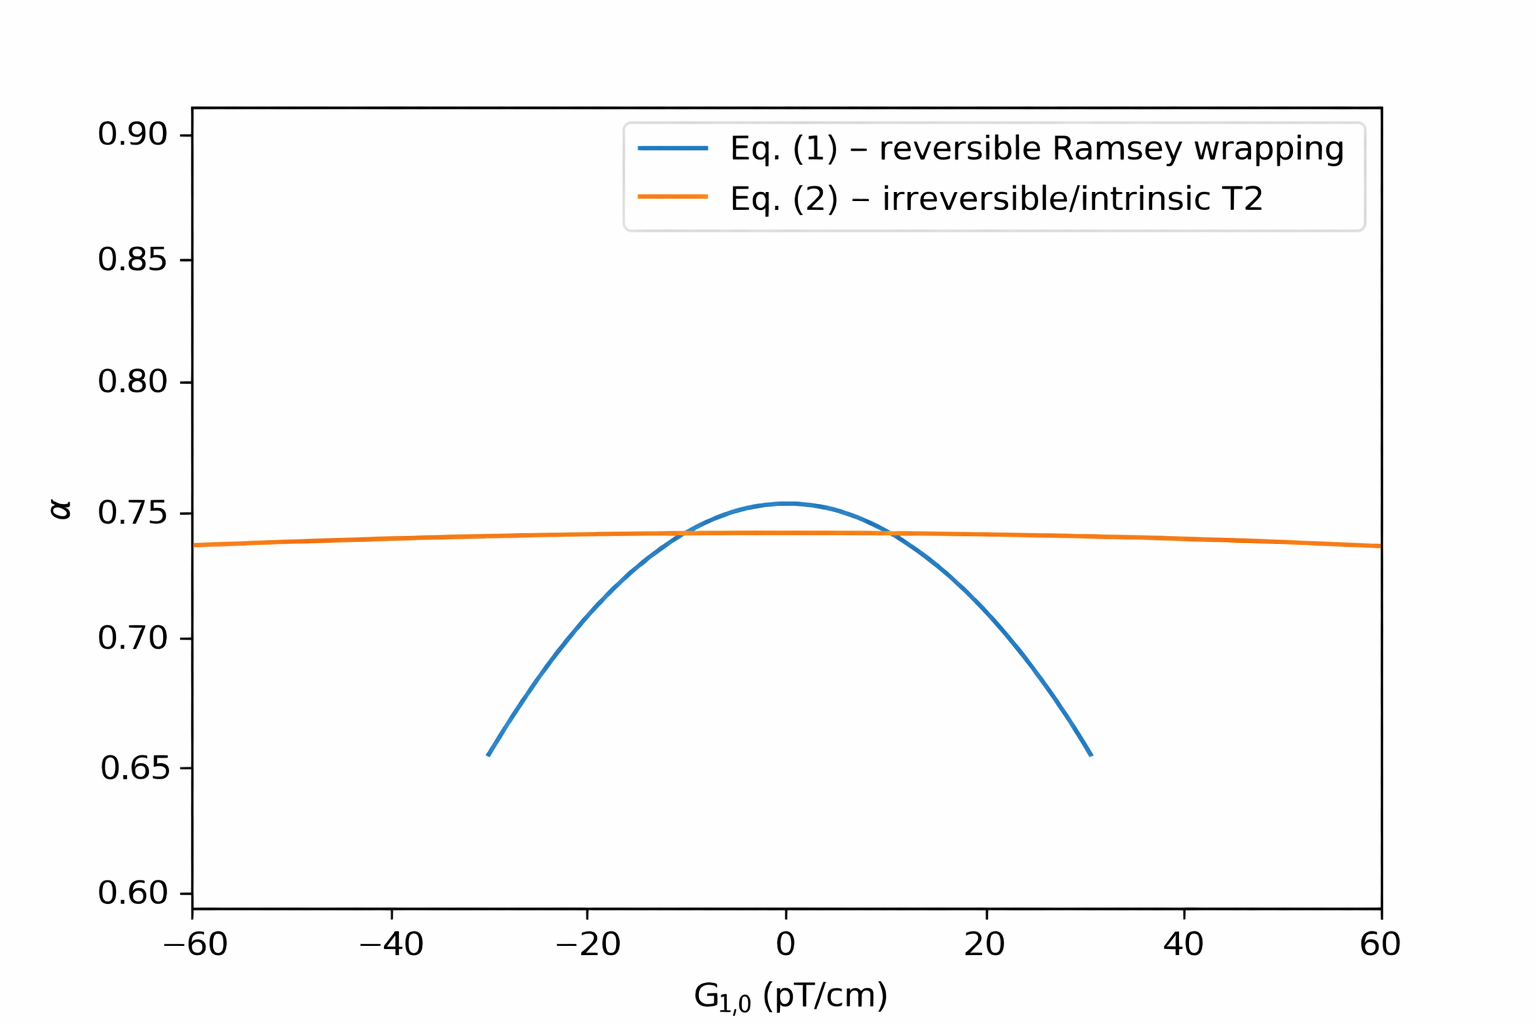
\includegraphics[width=0.90\linewidth]{Fig1Gravitational2.png}
  \caption{Calculated neutron visibility $\alpha$ after $T=180$~s as a
    function of the vertical gradient $G_{1,0}$, comparing
    gravitationally enhanced depolarization and intrinsic
    depolarization. The curves are obtained from the first-order
    gradient model using Eqs.~(\ref{eq:alphagrav}) and
    (\ref{eq:alphamag}) with parameters...???}
  \label{fig:g10_visibility}
\end{figure}

For the present design study, we adopted the working goal
\begin{equation}
  T_2 > 10{,}000~{\rm s}.
  \label{eq:t2goal}
\end{equation}
This corresponds to a visibility at $T=180$~s of
\begin{equation}
  \alpha > \alpha_0 \exp(-T/T_2)=\alpha_0\times 0.982.
  \label{eq:alphagoal}
\end{equation}

To estimate the corresponding first-order gradient requirements for
TUCAN, we used the requirement in Eq. (\ref{eq:alphagoal}) to place
constraints on $G_{1,0}$, $G_{1,-1}$, and $G_{1,1}$ via
Eqs. (\ref{eq:alphagrav}) and (\ref{eq:alphamag}), using the planned
cell dimensions $R=0.30$~m and $H=0.161$~m.  The results of the
calculation are shown in Table~\ref{tab:ggoal}
\begin{table}
  \begin{center}
    \begin{tabular}{ccl}
      quantity & upper bound & dominant constraint\\
               & (pT/cm) & \\\hline
      $\sqrt{G_{1,1}^2+G_{1,-1}^2}$ & $<$ 10.8 & intrinsic\\
      $G_{1,0}$ & $<$ 8.7 & gravitationally enhanced
    \end{tabular}
    \caption{Goals for first-order gradients based on requirement of
      maintaining magnetic inhomogeneity contribution to neutron
      visibility $\alpha>0.982\times\alpha_0$.\label{tab:ggoal}}
  \end{center}
\end{table}

Going beyond first order in magnetic gradients, we estimated
constraints on a general field $B_z(x,y,z)$ using two different
measures of inhomogeneity.  One measure was
\begin{equation}
  \Delta B_z = B_z^{\rm max}-B_z^{\rm min},
\end{equation}
where the maximum $B_z^{\rm max}$ and minimum $B_z^{\rm min}$ are the
extrema found anywhere within the measurement cell.  We alternatively
used the standard deviation $\sigma(B_z)$ of the values of $B_z$
within the measurement cell.  In the presence of a purely vertical
first-order gradient $G_{1,0}$, the quantities $\Delta B_z$ and
$\sigma(B_z)$ can be calculated analytically to be
\begin{equation}
  \Delta B_z = G_{1,0}H,
  \label{eq:dbz}
\end{equation}
and
\begin{equation}
  \sigma(B_z)=\frac{G_{1,0}H}{\sqrt{12}}.
  \label{eq:sbz}
\end{equation}
We used Eqs.~(\ref{eq:dbz}) and (\ref{eq:sbz}) to estimates
constraints on the more general $\Delta B_z$ and $\sigma(B_z)$ using
the constraint on $G_{1,0}$ described in Table~\ref{tab:ggoal}.  This
gives the requirements
\begin{equation}
  \Delta B_z<140~{\rm pT}
  \qquad\text{or}\qquad
  \sigma(B_z)<40~{\rm pT}.
  \label{eq:bzmetrics}
\end{equation}
A similar analysis can be conducted for the first-order horizontal
gradients of $B_z$, $G_{1,1}$ and $G_{1,-1}$, determining similar
results as Eqs.~(\ref{eq:dbz}) and (\ref{eq:sbz}).  The resultant
constraint turns out to be weaker, so we retained the constraints in
Eq.~(\ref{eq:bzmetrics}).

A further requirement comes from transverse magnetic fields. To lowest
order, the difference between the $^{199}$Hg comagnetometer frequency,
which senses $B_z$, and the neutron frequency, which senses
$|\vec{B}|$, differ by a factor $(1+\frac{\langle
  B_T^2\rangle}{2B_0^2})$, where $B_0$ is the nominal holding field,
and
\begin{equation}
  \langle B_T^2\rangle=\langle(B_x-\langle B_x\rangle)^2+(B_y-\langle B_y\rangle)^2\rangle
\end{equation}
where the averages are over the measurement cell volume.  A
requirement may be placed on $\langle B_T^2\rangle$ to ensure that
there is not a systematic difference between the comagnetometer and
neutron measured frequencies.  In the PSI experiment, $\langle
B_T^2\rangle < 1$~nT$^2$ was typically achieved.  As noted in
Ref.~\cite{bib:Abel2019} CHECK THAT IT SAYS THIS, requirements on
transverse fields are usually satisfied once the $B_z$ homogeneity is
sufficiently good.  Our studies confirmed this and
Eq.~(\ref{eq:bzmetrics}) was found to be sufficient.

\section{Design studies}\label{sec:designstudies}

\subsection{Assumed inhomogeneity}

To design the shim coil system, we needed to make an educated guess on
the likely inhomogeneity to be experienced prior to shimming.  We
assumed a 3 nT (max minus min) inhomogeneity within the central
1~m$^3$ volume surrounding the nEDM measurement cells.  This strategy
was based on similar studies performed in [Wolfgang K.'s MSc].  In
that case, the magnetic shielding of old ILL nEDM experiment, then at
PSI, was known to possess a native 3 nT/m gradient [find citation from
  Wolfgang K.'s MSc], and this was used as a benchmark.

Now that the MSR has been constructed, we expect the residual field
inhomogeneity within the central m$^3$ to fall within the 3 nT range
[Derek's MSR paper], with a significant probability of improvement
with more careful degaussing.  In the new n2EDM shield, the PSI
collaboration also demonstrated inhomogeneities of XX pT in the XX
m$^3$ region [cite first paper].  The homogeneity improved to XX pt in
XX m$^3$ after more detailed degaussing studies [cite Segarra paper]
and the degaussing time was substantially reduced.  The homogeneity in
the PanEDM experiment shield was demonstrated to be XX pT/m [find
  citation].  Other similarly sized MSRs have demonstrated even better
homogeneity of XX pT/m [cite Fierlinger plus Chinese people for Harbin
  room], [Fierlinger new shield].

\section{Design studies based on square coils in free space}

The software developed to perform design studies may be found at
\url{https://github.com/jmartin1454/squares}.  The software performs
the following tasks:
\begin{enumerate}
\item sets up an array of coils inscribed on a cube
\item sets up an array of fluxgates distributed throughout a smaller
  cube
\item calculates the matrix $M$ in $B=MI$ by setting each coil current
  $I$ in turn and measuring $B$ at each sensor position.
\item inverts the matrix, carefully excising the zero mode.
\item selects a target field $B_{\rm target}$ (uses the Pis library)
  and evaluates it at the fluxgate positions.
\item calculates $I_{\rm set}=M^{-1}B_{\rm target}$ and sets those
  currents on the cube
\item makes graphs of the resultant true field and graphs them in a
  few views (presently along axes), comparing with the target field.
\item performs statistics on the resultant residual magnetic field.
\end{enumerate}

The key development was a method to excise (remove) the problematic
zero mode, identified in \cite{bib:shomithesis}.  One additional and
generally useful development was the development of a library to
generate the functions $\Sigma_{\ell,m}$ and $\Pi_{i,\ell,m}$
($i=x,~y,~z)$ (defined in \cite{bib:psifields}).  The library is used
as a git submodule and may be found
at~\url{https://github.com/jmartin1454/Pis}.

We describe the details of some of the methods implemented in the
software, with a focus on the matrix algebra.  We then provide sample
results from this stage of the design.

\subsection{Geometry}

An example of the geometry constructed by the code is presented in
Fig.~\ref{fig:geometry}.
\begin{figure}
\begin{center}
  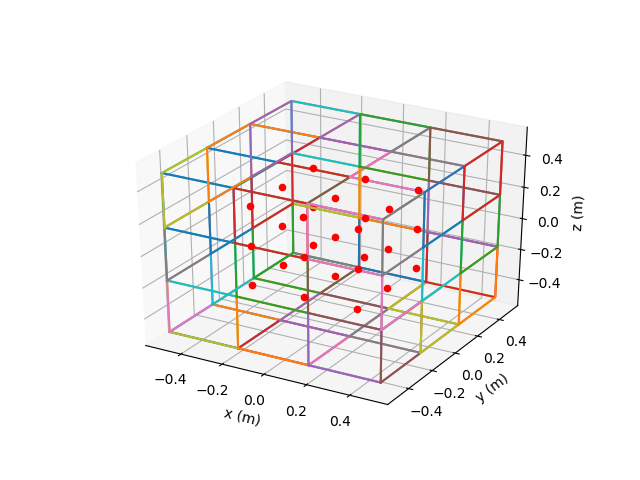
\includegraphics[width=\textwidth]{example-geometry.png}
  \caption{Example geometry.  Nine square coils are wound on each of
    the six faces of a 1~m cube (54 coils in total), represented by
    the colorful squares.  Twenty-seven fluxgate sensors (the red
    dots) are placed within a smaller 0.5~m cube, representing a
    volume of interest.\label{fig:geometry}}
\end{center}
\end{figure}
A cube defines the winding surface of the square coils.  The number of
square coils on each surface is selected by defining the integer
number of coils desired in each dimension.  In
Fig.~\ref{fig:geometry}, it is a $3\times 3$ ``coil cube''.

Three-axis sensors (which we can imagine as fluxgates) are placed
within a region of interest internal to the coil cube.  In
Fig.~\ref{fig:geometry}, 27~sensors are represented by the red dots
distributed within the smaller inner cube.  Each sensor has three axes
which measure $B_x$, $B_y$, and $B_z$.  So in total there are 81
sensor axes in this example.

\subsection{Matrix Methods, the Zero Mode, and how to remove it.}

\subsubsection{Matrix Methods}

Suppose that each coil carries a current $I_j$, where $j=1,...,c$ and
$c$ is the number of coils ($c=54$ in the example above).

The field $\vec{B}=(B_x,B_y,B_z)$ at each sensor position may be
calculated by summing the contributions from each coil.  In general
this field is easy to determine using the Biot-Savart Law, or, in this
case, the formula for a the magnetic field generated by a series of
straight-line segments.

Let the field at measured by each sensor axis be denoted $B_i$, where
$i=1,...,s$ and $s$ is the number of sensor axes.  (In the example of
Fig.~\ref{fig:geometry}, we have $s=81$.)  By superposition, the
magnetic field for each axis of each sensor is related to a sum of
contributions proportional to the current in each coil via
\begin{equation}
  B_i=\sum_{j=1}^cM_{ij}I_j.
\end{equation}
The matrix elements $M_{ij}$ are geometrical factors calculable by the
Biot-Savart Law or the formula of the magnetic field due to a
straight-line segment.

The equation may be written in a matrix notation as
\begin{equation}
  B=MI
\end{equation}
where $B$ is a column vector of $s$ values, $I$ is a column vector of
$c$ values, and $M$ is a matrix with $s$ rows and $c$ columns.  In the
example, $M$ would be an $81\times 54$ matrix, $B$ a column vector of
81 values and $I$ a column vector of 54 values.

The matrix elements $M_{ij}$ may be determined by applying a known
current to each coil ($j$) and determining the magnetic field at each
fluxgate axis ($i$).  The ratio of the sensed field to the set current
is the matrix element.

With the matrix $M$ in hand, the goal becomes to create a target field
$B=B_{\rm target}$ by setting the coil currents required which best
reproduce the required field.  The set currents can in principle be
determined from
\begin{equation}
  I_{\rm set}=M^{-1}B_{\rm target}.
  \label{eq:minv}
\end{equation}
The issue encountered is that the pseudoinverse of a non-square matrix
must be calculated.  The method to calculate the pseudoinverse
involves singular value decomposition.  This is analogous to inverting
a matrix by eigenvalue/eigenvector determination, for square matrices.

In singular value decomposition, the matrix $M$ is written as a
product of three matrices
\begin{equation}
  M=USV^T.
\end{equation}
Here $S$ is a diagonal matrix with the same dimension as $M$.  In the
example, it would be an $s\times c=81\times 54$ matrix.  The diagonal
values $S_{ii}$ are called the singular values.  If $c<s$, then there
are $c$ singular values, and any remaining for rows in $S$ (beyond the
$c$th row) are zero (up to the final $s$th row).  The matrices $U$ and
$V^T$ are square orthogonal matrices, containing the singular vectors.
The matrix $U$ has $s\times s=81\times 81$ values.  The matrix $V$ has
$c\times c=54\times 54$ values.

The diagonal elements $S_{ii}$ are positive and ordered in size with
$i=1$ being the largest and the last one, $i=c$, being the smallest.
It is easy to find the inverse of $S$, in principle.  Let $D$ be a
diagonal matrix of the same dimensions as $S$ ($s\times c=81\times
54$) whose diagonal elements are
\begin{equation}
  D_{ii}=1/S_{ii}.
\end{equation}
Then the inverse of $S$ is
\begin{equation}
  S^{-1}=D^T
\end{equation}
which will be a matrix of dimension $c\times s=54\times 81$.  With the
inverse of $S$ in hand, the pseudoinverse of $M$ may be calculated using
\begin{equation}
  M^{-1}=VS^{-1}U^T.
\end{equation}
Performing a check of dimensions, $V$ is $c\times c=54\times 54$,
$S^{-1}=D^T$ is $c\times s=54\times 81$, $U^T$ is $s\times s=81\times
81$, and so $M^{-1}$ will have the same dimensions as $S^{-1}$ and be
used as in Eq.~(\ref{eq:minv}) to calculate $I_{\rm set}$.

\subsubsection{Zero Mode}

While this calculation works in principle, in practice it can have
problems.  For coils with overlapping currents inscribed on a cube,
there is always one mode of applying the same magnitude current to all
$c$ coils, which gives rise to exactly zero net current and hence
$\vec{B}=0$ in all space.  This mode appears in the singular value
decomposition as
\begin{equation}
  S_{cc}=0,
\end{equation}
where $c=54$ in the example.  That is, the smallest singular value
will always be identically zero.  Since the singular values are
ordered in size, it will always appear in the last value in the $S$
matrix.  The singular mode in $V^T$ corresponding to this singular
value will appear in the last row of $V^T$.  It will have values all
of the same magnitude, corresponding to applying all the same
currents, up a to sign convention on the current.  We refer to this
mode as the ``zero mode'' because it corresponds to zero net current
generating zero magnetic field.

Even in the case of real wires that do not overlap perfectly, we will
nonetheless have $S_{cc}<<S_{jj}$ for $j<c$.

This poses a problem for finding $D_{cc}=1/S_{cc}$ which will
correspondingly have a much larger value than all the other elements
in the $D$ matrix.

Even in the case where $S_{cc}$ is not exactly zero, it leads to
problems in applying Eq.~(\ref{eq:minv}) to calculate the set currents
$I_{\rm set}$.  One strategy is to press forward and ignore the
problem of the small singular value, calculating $M^{-1}$ as described
above.  This generally will result in unstable values in $I_{\rm
  set}$.  By this we mean that small changes in $B_{\rm target}$ will
result in large changes in $I_{\rm set}$.  A smaller dimensional
example of this problem may be found in~\cite{bib:gregorcic} which has
been translated into python in~\cite{bib:test}.  Ultimately these
problems result from having one small singular value, for this system.

The zero singular value signifies an ill-conditioned problem.  It also
shows up in the condition number, defined as $S_{11}/S_{cc}$ which in
this case is very large, or infinite in the ideal case of perfectly
overlapping currents.

There are a number of strategies that can be used to treat
ill-conditioned systems:
\begin{itemize}
  \item Matrix regularization, for example Tikhonov
    regularization~\cite{bib:franke}.  A transformation is made on the
    $S_{ii}$ to make them more similar in magnitude.
  \item Preventing the problematic mode from occuring by constraining
    the allowed currents.  In Ref.~\cite{bib:shomithesis} this was
    done by wiring two coils together (in a six-coil system) so that
    the zero mode could not be generated.  While this process was
    successful in the six-coil system, it is not obvious how to
    generalize the process to a system with a larger number of coils.
  \item Cutting out the problematic mode (truncation).  In this
    method, the zero mode and its corresponding singular vector are
    thrown away.  This is likely the simplest generalization of the
    process followed in Ref.~\cite{bib:shomithesis}, although a few
    other possible methods were also suggested in that reference.
\end{itemize}
We now focus on this third solution.

\subsubsection{Truncation}

For coils, $S_{cc}$ can be very small relative to the other $S_{ii}$
with $i<c$.  The systematic way in which to eliminate $S_{cc}$ and its
associated singular vector is called truncation.

Let $D'$ be a reduced dimension diagonal matrix, where the last column
(the one with the bad singular value in it) has been removed.  The
matrix $D'$ is still diagonal and we keep its other diagonal elements
as before $D'_{ii}=1/S_{ii}$ however now with the final value being at
index $i=c-1$.  The matrix $D'$ will then be of dimension
$s\times(c-1)=81\times 53$.

It is also necessary to remove the singular vector corresponding to
the zero mode from $V^T$.  It is in the last row of $V^T$.  Cutting
the last row results in the modified matrix $(V^T)'$ which becomes
dimension $(c-1)\times c=53\times 54$.

The modified pseudoinverse may then be calculated from
\begin{equation}
  (M^{-1})'=((V^T)')^T(D')^TU^T.
\end{equation}
Performing a check on the rows and columns of each matrix shows that
$((V^T)')^T$ is $54\times 53$, $(D')^T$ is $53\times 81$, and $U^T$
retains its size of $81\times 81$.  The matrix $(M^{-1})'$ then retains
the same dimensions as $M^{-1}$, being a $54\times 81$ matrix.

The set currents can be determined using the new inverse as
\begin{equation}
  I_{\rm set}=(M^{-1})'B_{\rm target}
\end{equation}
and the currents will be well-behaved under small changes in $B_{\rm
  target}$.

Most codes that can perform matrix manipulations of this sort have
built-in functions to perform the truncation.  For example, in python,
the function numpy.linalg.pinv() will automatically truncate singular
values and vectors based on a set precision.  By default, this
function cuts singular values smaller than the machine precision.  For
perfectly overlapping coils, this means that the zero mode is
automatically cut.

In developing the present coil-design code~\cite{bib:code}, care has
been taken to deal explicitly with each matrix as described above.
This gives a better understanding of each matrix.  The hope is that
the decision whether or not to cut the zero mode (or in the case of
realistic current paths, the slightly non-zero mode) can then be made
by the user, when more realistic coil systems are eventually studied.

\subsection{Quantitative comparison to requirements}

As discussed in Ref.~\cite{bib:jeffnote}, and as mentioned in
Section~\ref{sec:req}, the chief requirements are:
\begin{itemize}
\item $\Delta B_z\equiv B_z^{\rm max}-B_z^{\rm min}<140~{\rm pT}$,
\item $\sigma(B_z)<40~{\rm pT}$, and
\item $\langle B_T^2\rangle<0.1$~nT$^2$.
\end{itemize}

One difficulty encountered in deciding whether a given design meets
these requirements is how to normalize the anticipated
inhomogeneities.  Since we do not know the actual field distribution
expected in the MSR, we can only guess at the extent of the
inhomogeneity that might need to be dealt with.

The strategy pursued here is to normalize our ignorance of the
homogeneity to the scale of inhomogeneity experienced in other
magnetically shielded enclosures.  A similar strategy has been pursued
in Ref.~\cite{bib:wkthesis}.  In that case, the magnetic shielding of
PSI, which is known to possess a native 3~nT/m gradient, was used as a
benchmark.  This was used to motivate placing a requirement on
randomly generated fields within a $1\times 1\times 1$~m$^3$ region of
interest fall within a range of 3~nT.  The alkali atom magnetometers
studied in Ref.~\cite{bib:wkthesis} were then studied in relation to
their performance in these fields, and their ability to extract the
relevant vertical gradients, which contribute to false EDM effects.
For example, a genetic algorithm was used to decide the optimal
magnetometer positions to best constrain the $G_{\ell,0}$.

A key finding in this study was that $\ell>3$ did not contribute
strongly to the false EDM.  This is, in part, because of the
normalization volume and range of magnetic fields permitted.

In our study, a similar strategy is adopted.  The maximum and minimum
values of the target field ($B_z$) in a $1\times 1\times 1$~m$^3$ cube
are determined.  The range of $B_z$ (maximum minus minimum) is then
required to be 3~nT, as in~\cite{bib:wkthesis}, and all $B_z$ values
within the volume renormalized accordingly.  This field is then
decided to be ``reasonable'' as a possible inhomogeneity that might be
encountered in the eventual EDM experiment.

Within this normalization volume are placed the two (upper and lower)
EDM measurement cells.  The cells are assumed each to be 16~cm in
height and 30~cm in radius.  The cells are separated by an 8~cm
central electrode.  Statistics on the target $B_z$ field (prior to
correction) and the residual $B_z$ (corrected by the coils) are
calculated within the cell volumes.

\begin{table}
  \begin{center}
    \begin{tabular}{ccccccc}
      $(\ell,m)$ & \multicolumn{2}{c}{$\Delta B_z$} & \multicolumn{2}{c}{$\sigma(B_z)$} & \multicolumn{2}{c}{$\langle B_T^2\rangle$}\\
      or &  \multicolumn{2}{c}{(pT)} & \multicolumn{2}{c}{(pT)} & \multicolumn{2}{c}{(nT$^2$)} \\\cline{2-7}
      dipole & before & after & before & after & before & after \\
      & correction & correction & correction & correction & correction & correction \\\hline
      (1,0) & 455 &  6 & 140 & 0.6 & 0.26 & $3\times 10^{-6}$ \\
      (1,1) &1790 &106 & 458 & 9 & 0.36 & $2\times 10^{-4}$ \\
      (2,0) & 500 & 58 & 106 & 7 & 0.04 & $4\times 10^{-4}$ \\
      (2,1) & 700 & 16 & 120 & 2 & 0.02 & $5\times 10^{-5}$ \\
      (2,2) &1065 &116 & 230 &12 & 0.17 & $4\times 10^{-4}$ \\
      dipole 1 &1140&$\boxed{232}$ & 244 &14 & 0.53 & $7\times 10^{-4}$ \\
      dipole 2 upper&500& 20 & 109 & 3 & 0.47 & $3\times 10^{-5}$ \\
      dipole 2 lower&220& 17 &  50 & 3 & 0.47 & $3\times 10^{-5}$ \\
      dipole 3 upper&870& 37 & 187 & 8 & 0.16 & $1\times 10^{-4}$ \\
      dipole 3 lower&400& 41 &  87 & 4 & 0.16 & $1\times 10^{-4}$ \\
      (3,1) & 200 & 61 &  31 & 6 & 0.004& $1\times 10^{-4}$ \\
      (3,3) & 340 & 65 &  61 & 5 & 0.02 & $2\times 10^{-4}$ \\
      (4,2) & 123 & 59 &  14 & 6 & 0.0005&$2\times 10^{-4}$ \\
      \hline
      goal & & 140 & & 40 & & 0.1 \\
    \end{tabular}
    \caption{Trials using the $3\times 3$ coil/fluxgate system to
      counteract various applied fields.  The only entry not meeting
      requirements has been highlighted.\label{tab:trials}}
  \end{center}
\end{table}

While Ref.~\cite{bib:wkthesis} considered a broad range of possible
field configurations, we focused on a few different orders of
$G_{\ell,m}$ and some dipole fields.  Table~\ref{tab:trials} details
the various target field configurations that that were studied.

In general, vertical gradients $(\ell,m=0)$ are well-compensated
compared to gradient possessing large variations in $B_z$ in the
transverse directions $(\ell,m=\ell)$.  This is in part because the
cells are wider than they are tall.  It seems also that the gradient
suppression is not as good generally for these modes for this design.
Nonetheless, all $(\ell,m)$ modes meet the requirements.

The dipole fields considered were as follows:
\begin{itemize}
  \item Dipole 1 represents the dipole location and moment presented
    in Eqs.~(\ref{eq:dipoleposition}) and (\ref{eq:dipolemoment}),
    respectively, and with fields as shown in Fig.~\ref{fig:dipole}.
  \item Dipole 2 has the same vector moment, pointing in the $+z$
    direction, but its position has been moved to the ceiling center
    at $(x_d,y_d,z_d)=(0,0,1.2)$~m.  In this position, the dipole has
    a different effect on the upper and lower cells and we list their
    results separately in Table~\ref{tab:trials}.  (However, their
    $B_T$ results are presented as averages of the upper and lower
    cells.)
  \item Dipole 3 has the same position as dipole 2, but the moment has
    been oriented along the $+x$ direction $\vec{p}=(1,0,0)$~Am$^2$.
\end{itemize}

As shown in Fig.~\ref{fig:dipole}, dipole 1 generates a strong and
varying $\partial B_z/\partial x$ across the cells.  In this way it is
quite similar to the $G_{1,1}$ multipole.  This was the only
configuration considered that did not meet the $\Delta B_z$
requirement, although it did meet the $\sigma(B_z)$ requirement.

To test whether this failure was due to the dipole nature of the
field, or the strong $\partial B_z/\partial x$ field generated by it,
the dipole 2 and dipole 3 configurations were created.  Dipole 2 gives
a similarly strong $\partial B_z/\partial z$ field, which differs in
the upper and lower cells.  This is easily corrected.  Dipole 3 gives
a relatively strong $\partial B_z/\partial x$.  By symmetry, its
behavior is the same as the $B_x(0,0,z)$-dependence exhibited by
dipole 1.  Interestingly, despite having a relatively strong $\partial
B_z/\partial x$, it is corrected sufficiently well to meet the
requirement.

The worst result seen in Table~1, indicated by the boxed value, seems
to be driven in part by a particularly pathological $\partial
B_z/\partial x$.  While it does not meet the requirement set in
Ref.~\cite{bib:jeffnote} that $\Delta B_z<140$~pT, recall that this
requirement was set based on a $G_{1,0}$, {\it i.e.} a $\partial
B_z/\partial z$ vertical gradient, and that the requirements on
horizontal gradients were generally much looser.  In the end, we
suggest that the $3\times 3$ array is likely sufficient to meet the
neutron $T_2$ requirements, for the geometry factors considered here.

Finally, the $\langle B_T^2\rangle$ are also always met.  The response
to pure transverse gradient fields $G_{\ell,\pm(\ell+1)}$ was not
studied yet, in part due to the normalization scheme being focused on
the vertical field $B_z$.  But the reduction for pure transverse
gradients could be expected to be similar in magnitude to the
suppression of transverse gradients affecting $B_z$.  For example the
suppression of $G_{1,2}$ might be similar in scale to the suppression
of $G_{1,1}$ which generates transverse gradient $\partial
B_z/\partial x$, but not as large as the suppression of $G_{1,0}$,
which generates $\partial B_z/\partial z$.  For dipoles 2 and 3, it
should also be noted that the $\langle B_T^2\rangle$ was not
calculated separately for each cell, rather the results in the table
are averaged over the two cells.

\section{Design concepts}\label{sec3}

?

\subsection{Current supply for shim-coil operation}

The square shim-coil system requires independent current control for
each coil, since each target field pattern is produced by applying a
calculated set of currents to the full coil array. For the prototype
system, the required currents are modest, typically at the level of a
few tens of milliamperes. However, stability and reproducibility are
important because the magnetic field produced by each coil is
proportional to the applied current. Therefore, current drifts would
directly appear as magnetic-field drifts during mapping or shimming
measurements.

The shim coils are driven using a modular 64-channel bipolar current
supply developed for precision magnetic-field control
\cite{bib:AhmedCurrentSupply2026}. The 64-channel design provides
enough channels for the 54-coil square-shim array, with additional
spare channels available for testing and future expansion. Each
channel can supply a bipolar current of approximately $\pm
40~\mathrm{mA}$, which is sufficient for the current range required by
the shim-coil setpoints.

The current supply consists of one power distribution board and four
16-channel current-source boards, as shown in
Fig.~\ref{fig:current_supply}. The current setpoints are programmed
digitally and converted to analog reference voltages using 16-bit
digital-to-analog converters. Each output channel then uses a feedback
circuit with a precision sense resistor to regulate the coil
current. The bipolar output is useful for shim operation because the
calculated current for a given coil may be positive or negative
depending on the desired correction field or harmonic-gradient mode.

The performance of this current supply was characterized separately in
Ref.~\cite{bib:AhmedCurrentSupply2026}. Long-term measurements showed
current stability at the $10^{-5}$ level over several hours, which is
better than the stability requirement for shim-coil operation. A
scale-model coil experiment also demonstrated that the supply can
reproduce calculated current patterns accurately. In the present work,
this current supply is used to apply the matrix-calculated setpoints
for individual-coil tests and harmonic-mode measurements.

\begin{figure}[tbp]
\centering
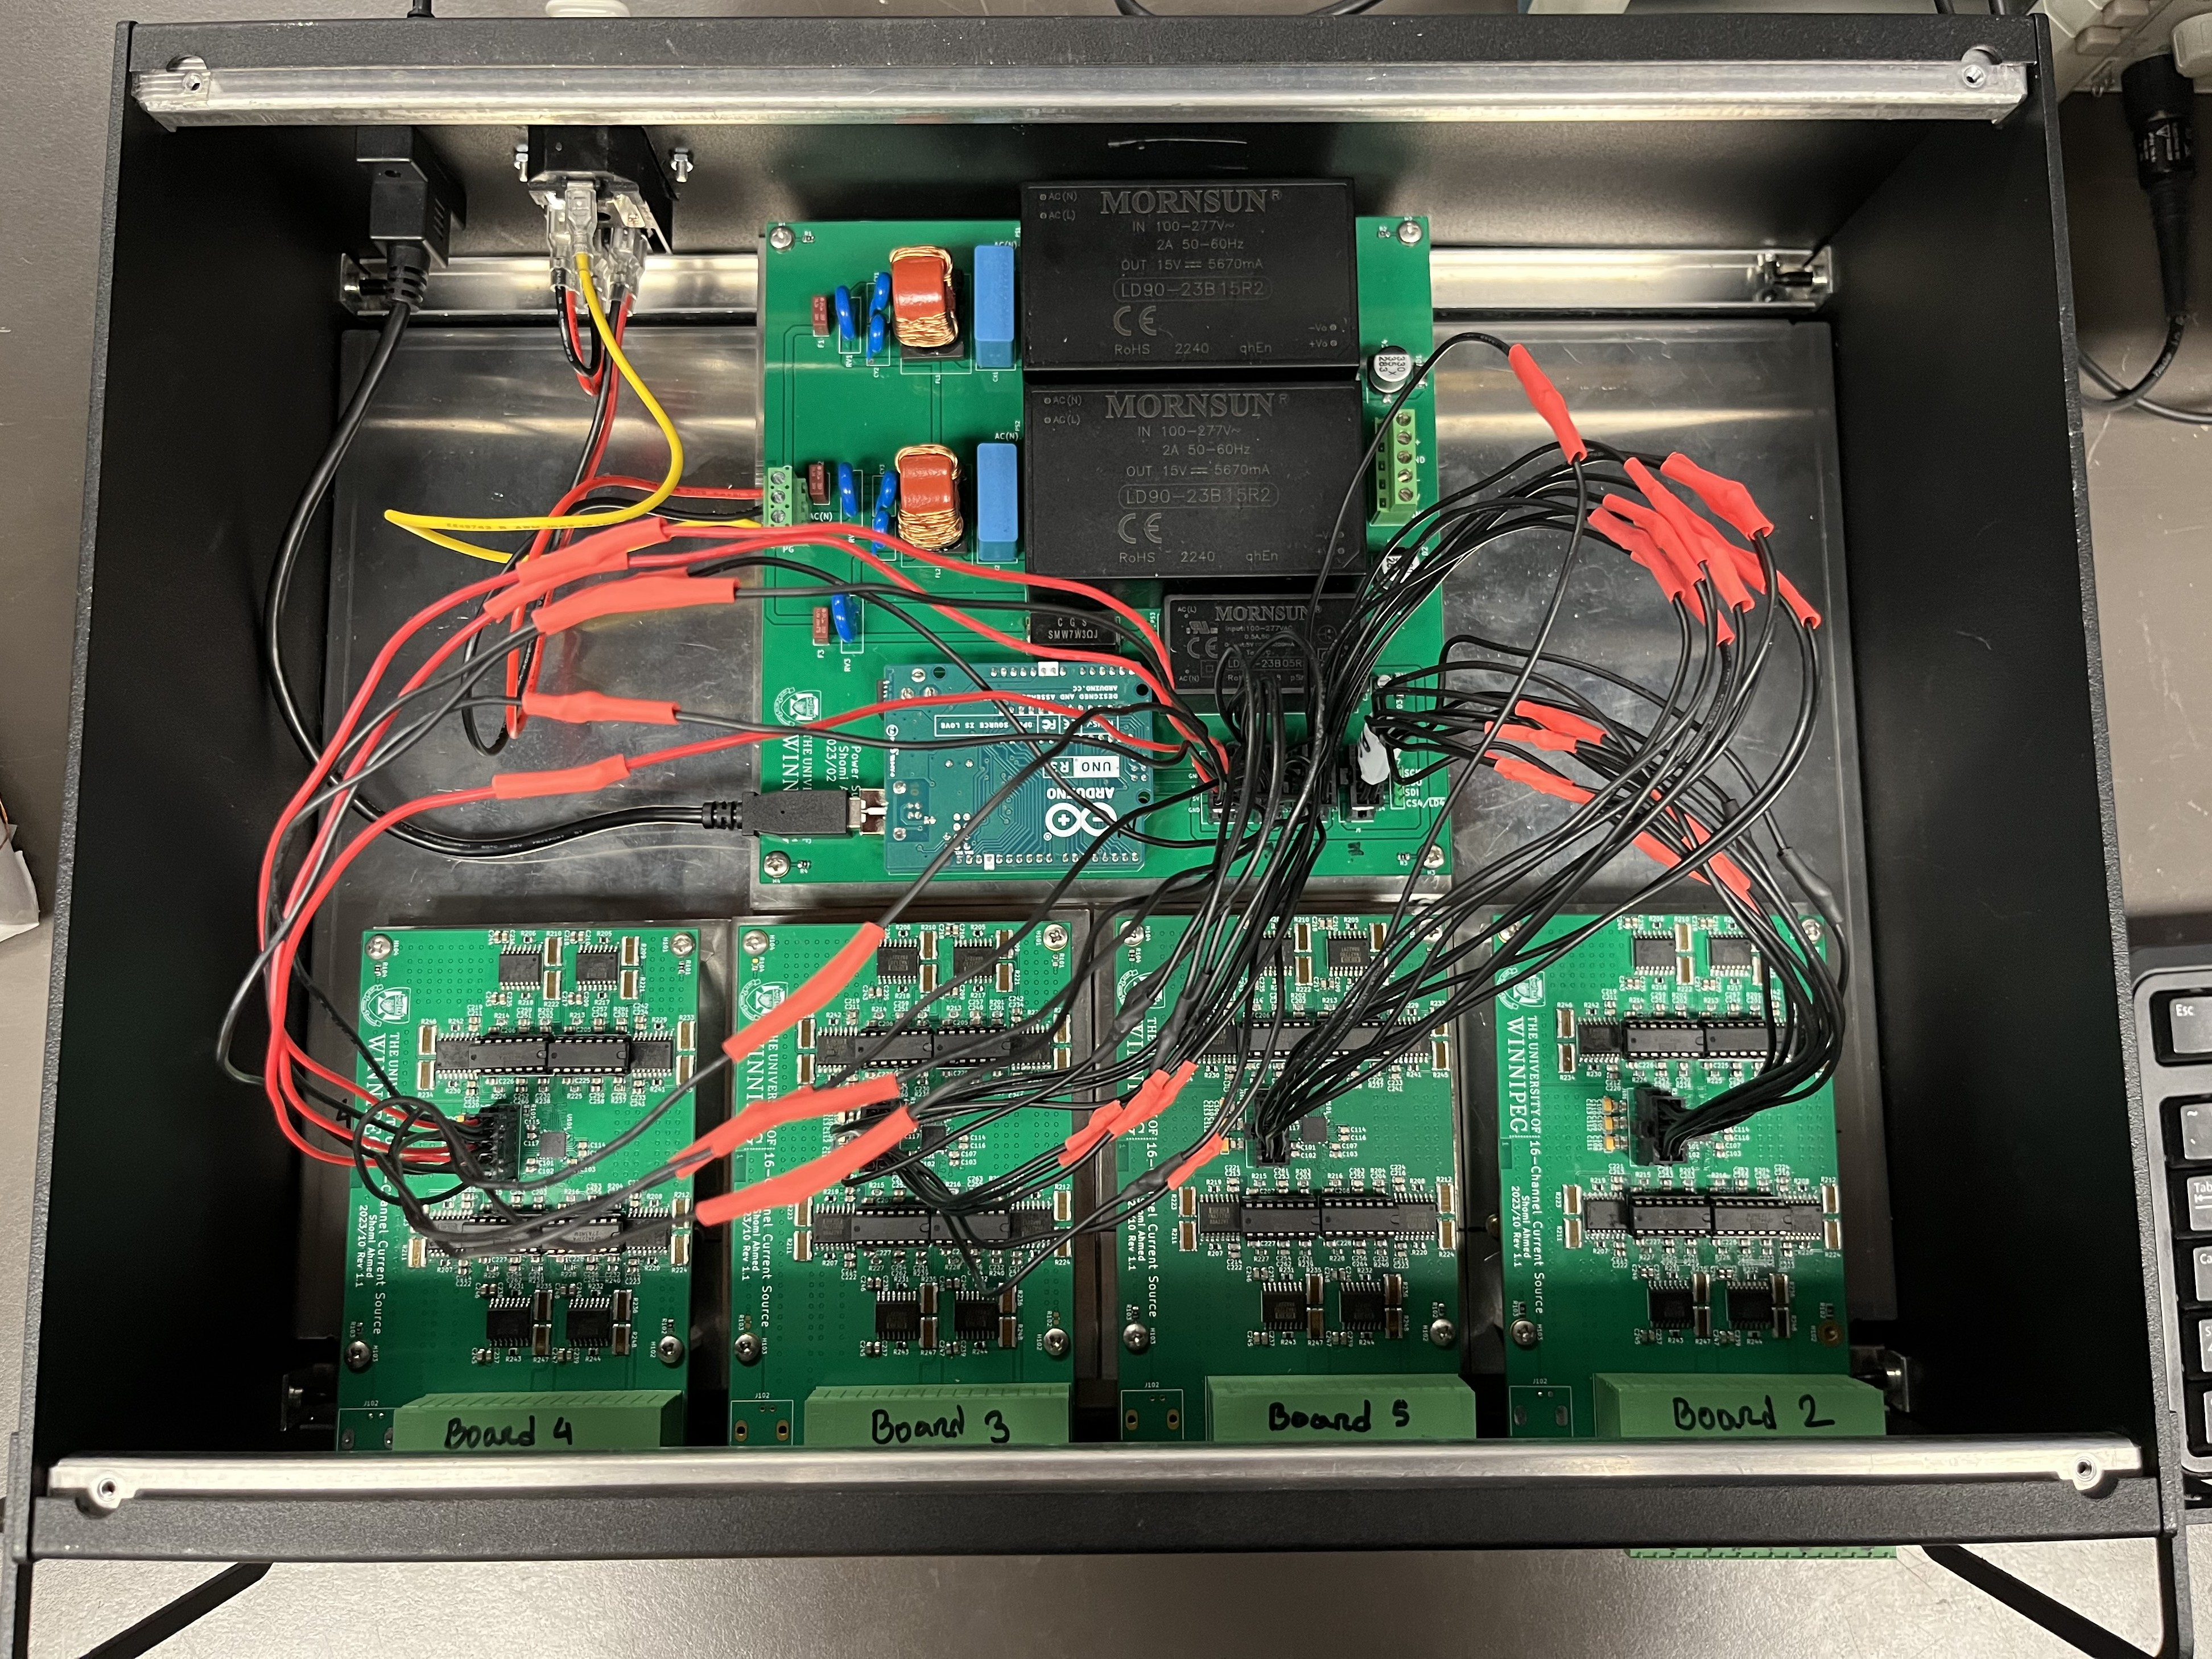
\includegraphics[width=0.75\linewidth]{current_supply_enclosure.png}
\caption{Fully assembled 64-channel bipolar current supply used to
  drive the shim-coil array. The system consists of one
  power/distribution board and four 16-channel current-source boards
  mounted inside a shielded enclosure.}
\label{fig:current_supply}
\end{figure}

\section{Construction and installation}\label{sec6}

\subsection{Panel fabrication and coil winding}

The shim-coil array was implemented on six $4'\times4'$ corrugated
plastic (Coroplast) sheets, chosen because it is lightweight, rigid,
and easy to machine and handle. The coil geometry was marked directly
on the sheet. After the layout was verified, grooves were cut to hold
the wire placement: grooves across the ribs were made using a thin
circular-saw blade, while grooves along the ribs were made using a
knife.

Each square coil was wound using 30~AWG magnet wire with three turns
per coil, which provides sufficient field amplitude at modest
operating currents. On each panel, the lead wires were routed so that
they converge at a common exit point, simplifying cable
organization. To avoid blocking the feed throughs in the walls of the
MSR, circular cutouts were made in the required locations on the
corroplast sheets.

\subsection{Installation inside the MSR and cabling}

The 6 prototype panels were secured on the center of the MSR interior
walls mostly using tapes and mechanical fasteners when mount points
where available.Tape was used to allow easy removal of prototype
panels at a later date.  For each face, nine coils require eighteen
conductors (two leads per coil). Ethernet cables were used as
convenient multi-conductor bundles, with three cables per face and all
cables routed through the MSR extrusions to a centralized location for
easier connection to the current source. This organized routing and
labeling is essential for reliable commissioning, mapping, and
repeatable generation of harmonic modes.

\begin{figure}[tbp]
  \centering
  \includegraphics[width=0.46\linewidth]{Fig5-smaller.png}
  \caption{Prototype square shim coils installed inside the TUCAN
    MSR. The full system comprises 54 coils arranged as nine coils on
    each of the six faces of the cubic structure. In this photograph,
    the side-wall, ceiling, and far-end panels are visible, while the
    floor and door-side panels are outside the field of view. The MSR
    provides passive magnetic shielding using high-permeability
    mu-metal.}
  \label{fig:msr_prototype_install}
\end{figure}


\section{Mapping results}\label{sec7}

Magnetic field mapping of the shim-coil system was carried out to
verify proper coil operation and to evaluate the ability of the system
to generate controlled magnetic-field gradients relevant to the TUCAN
nEDM experiment. Measurements were performed along the central scan
axis using a three-axis fluxgate magnetometer. The probe was moved
from $-99.5$~cm to $+100.5$~cm in steps of 10~cm, where $z=0$
corresponds to the center of the system. At each position,
measurements were taken for both positive and negative applied
current. The shim-coil field was then obtained from the current-odd
component,
\begin{equation}
  B_{\mathrm{coil}}=\frac{B(+I)-B(-I)}{2},
\end{equation}
which suppresses constant backgrounds and slow drifts. The same
procedure was used both for individual-coil measurements and for the
harmonic-mode measurements described below.


\subsection{Verification of individual shim coils}

Each of the 54 shim coils was mapped individually in order to verify
the electrical connections and magnetic response. The measurement
procedure described above was applied to each coil in turn using $\pm
40$~mA. The magnetic-field profiles measured for all individual coils
were in good agreement with the simulated
fields. Figure~\ref{fig:singlecoil} shows three representative
examples. In each case, the measured $B_x$, $B_y$, and $B_z$
components reproduce the main features of the corresponding COMSOL
profiles, confirming correct coil connectivity and magnetic
response. These results show that all shim coils were functioning as
expected and were suitable for producing controlled magnetic-field
gradients.
\begin{figure}
  \centering

  \begin{minipage}[t]{0.50\textwidth}
    \centering
    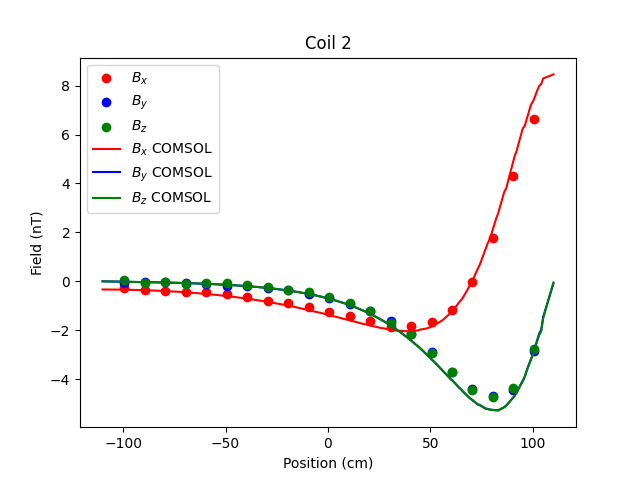
\includegraphics[width=\linewidth]{coil2.png}
    \vspace{1mm}
    {\scriptsize (a) Coil 2}
  \end{minipage}\hfill
  \begin{minipage}[t]{0.50\textwidth}
    \centering
    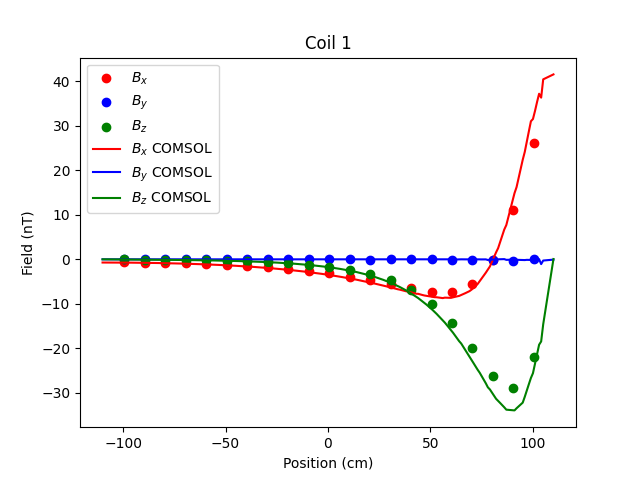
\includegraphics[width=\linewidth]{coil1.png}
    \vspace{1mm}
    {\scriptsize (b) Coil 1}
  \end{minipage}

  \vspace{2mm}

  \makebox[\textwidth][c]{%
    \begin{minipage}[t]{0.50\textwidth}
      \centering
      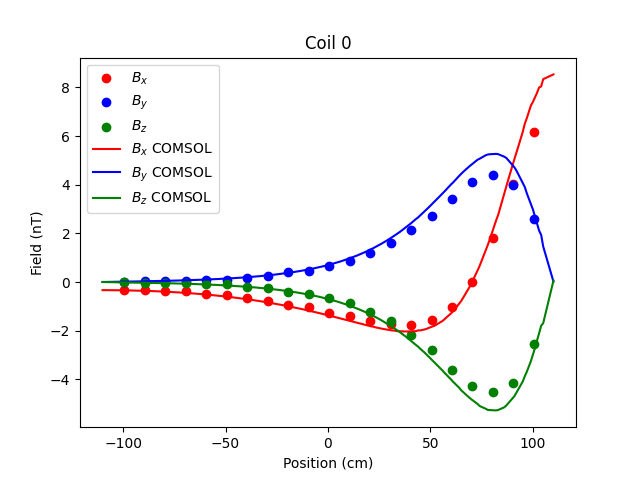
\includegraphics[width=\linewidth]{coil0.png}
      \vspace{1mm}
      {\scriptsize (c) Coil 0}
    \end{minipage}
  }

  \caption{Measured magnetic-field components $B_x$, $B_y$, and $B_z$
    along the central scan axis for three representative individual
    shim coils (coils 2, 1, and 0), compared with the corresponding
    COMSOL calculations. The measured profiles are in good agreement
    with the simulated fields, confirming proper coil connectivity and
    magnetic response.}
  \label{fig:singlecoil}
\end{figure}

\subsection{Mapping of the $G_{1,0}$ gradient mode}

After verifying the individual coils, the shim-coil system was
configured to generate the linear gradient mode $G_{1,0}$. The
coil-current setpoints were calculated using two approaches. In the
first, free-space Biot--Savart calculations were used. In the second,
the coil-current setpoints were obtained from COMSOL-based
calculations that include the surrounding magnetic environment
\cite{bib:comsol}.

The measured magnetic-field components $B_x$, $B_y$, and $B_z$ show good agreement in spatial shape with the simulated fields along the central scan axis. Figure~\ref{fig:G10map} shows the measured and simulated field components. An overall amplitude difference between measurement and simulation was corrected by applying a single scaling factor derived from the $B_x$ component. The fitted scaling factor for the $G_{1,0}$ mode was 0.937.

After applying this scaling factor, the residual field in the dominant measured component was reduced substantially in the central region of interest. In particular, the variation in the dominant component was reduced from about $2.2\times10^{4}$~pT before correction to about $1.8\times10^{2}$~pT after correction, corresponding to a reduction by a factor of more than 100. Figure~\ref{fig:G10residual} shows the scaled residual field along the central scan axis. These results indicate that the shim-coil system is able to strongly suppress large gradient fields and support the expectation that room-scale gradients of order 10~nT can be reduced to below the target range relevant for TUCAN operation.

\begin{figure}[tbp]
  \centering
  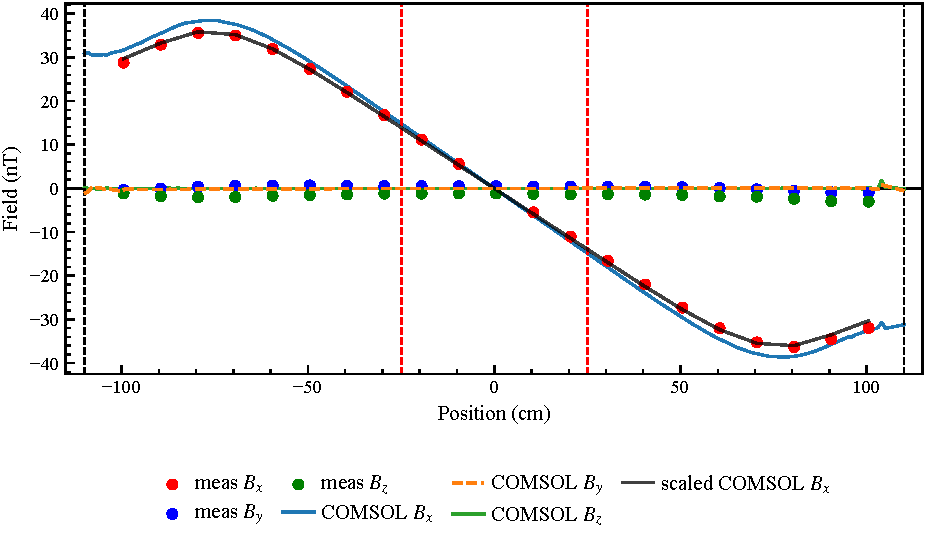
\includegraphics[width=0.92\linewidth]{G10.pdf}
  \caption{Measured and simulated magnetic-field components $B_x$, $B_y$, and $B_z$ along the central scan axis for the linear gradient mode $G_{1,0}$. The measured fields are compared with COMSOL-based simulations using the same coil-current setpoints. A single scaling factor of 0.937, derived from the $B_x$ component, was applied to the simulated field.}
  \label{fig:G10map}
\end{figure}

\begin{figure}[tbp]
  \centering
  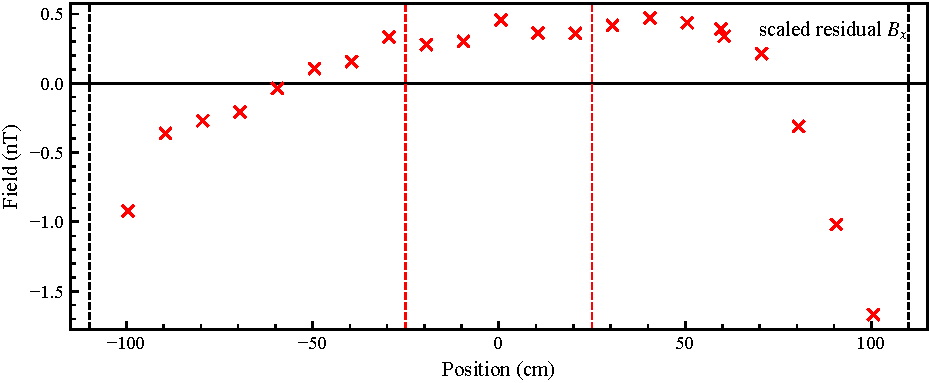
\includegraphics[width=0.92\linewidth]{G10_scaled.pdf}
  \caption{Scaled residual field for the $G_{1,0}$ mode along the central scan axis after applying the common ';scaling factor to the simulated field.}
  \label{fig:G10residual}
\end{figure}
\subsection{Generation of higher-order harmonic modes}

In addition to the $G_{1,0}$ mode, the shim coil system was used to generate higher-order harmonic modes, including $G_{1,2}$ and $G_{2,1}$. For these measurements, the coil current setpoints were calculated using COMSOL-based response matrices. Magnetic field profiles measured along the central scan axis for these modes are shown in Fig.~\ref{fig:residuals_G12_G21}.
\begin{figure}[tbp]
  \centering
 \makebox[\linewidth][c]{%
  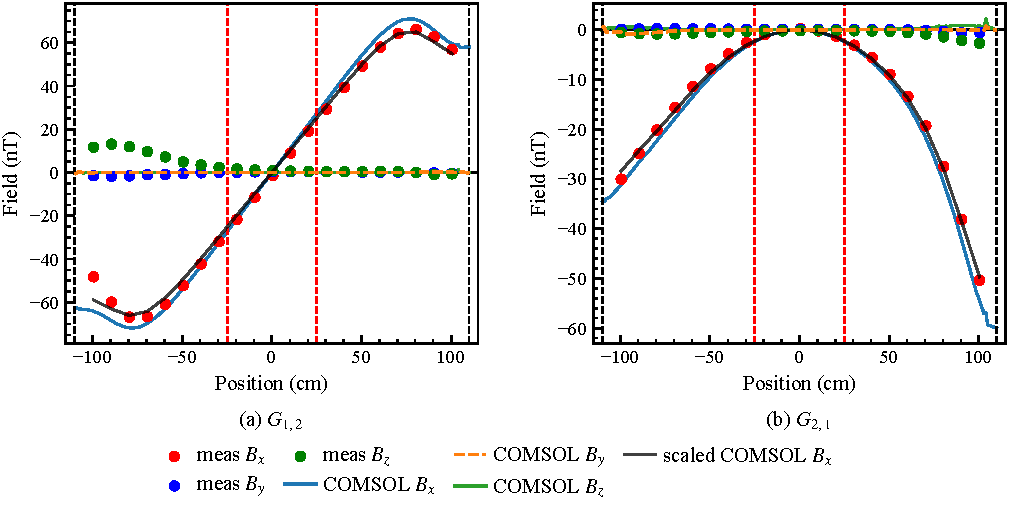
\includegraphics[width=1.16\linewidth]{G12_G21_combined.pdf}
}
  \caption{Measured and COMSOL-simulated magnetic field components $B_x$, $B_y$, and $B_z$ along the central scan axis for the $G_{1,2}$ and $G_{2,1}$ gradient modes generated using COMSOL-derived current setpoints.}
  \label{fig:residuals_G12_G21}
\end{figure}

The measured field shapes for the higher-order modes follow the expected spatial structure of the corresponding harmonic fields. These measurements demonstrate the flexibility of the shim coil system and its capability to generate a range of gradient field configurations relevant for magnetic field optimization in the TUCAN nEDM experiment. A detailed quantitative analysis of higher-order modes is left for future work.

\section{Discussion and Conclusion}\label{sec8}

The magnetic field mapping results demonstrate that the square shim coil system can reliably generate controlled gradient fields inside the magnetically shielded room for the TUCAN nEDM experiment. Central-axis scans of the three field components provide a direct validation of the coil response and of the current setpoints used for field generation.

For the $G_{1,0}$ configuration, the measured field components $B_x$, $B_y$, and $B_z$ reproduce the simulated spatial structure along the scan axis. An overall amplitude difference between measurement and simulation was accounted for using a single normalization factor derived from the $B_x$ component, and the residual field after normalization is reduced to approximately $\pm 0.5~\mathrm{nT}$ over the region of interest. These results show that the shim coil system can generate and tune the dominant vertical gradient field required for field optimization.

Higher-order harmonic modes were also generated using COMSOL-derived current setpoints. The measured profiles follow the expected harmonic structure and remain consistent with the simulated field components along the central scan axis, demonstrating the flexibility of the shim coil system and its capability to produce a range of gradient-field configurations relevant for magnetic field optimization in the TUCAN nEDM experiment.

Future work will extend this characterization beyond the central axis by analyzing field maps acquired in additional mapping holes and through the MSR door, and by carrying out a more detailed quantitative evaluation of higher-order mode performance, repeatability, and stability.


\section*{Acknowledgments}
The authors would like to thank all members of the TUCAN collaboration, as well as the technical and support staff at TRIUMF, for their contributions to this work. The authors also gratefully acknowledge CMC Microsystems for the provision of CAD software. Funding for this work and the TUCAN collaboration was supported by the Canada Foundation for Innovation; the Canada Research Chair program; the Natural Sciences and Engineering Research Council of Canada (NSERC) SAPPJ2016-00024, SAPPJ-2019-00031 and SAPPJ-2023-00029; Japan Society for the Promotion of Science (JSPS) KAKENHI grants 18H05230 and 20KK0069; JSPS KENHI grants 17K14307, 19K23442, 20K14487, 21K13940, 22H01236; RCNP CORENet; the Universidad Nacional Autónoma de México DGAPA program PASPA; and grant PAPIIT AG102023..

\bibliographystyle{elsarticle-num}
\bibliography{shim_coil_refs}

\end{document}
